\documentclass[11pt]{article}
\usepackage[spanish]{babel}
\usepackage[utf8]{inputenc}
\usepackage{amsmath}
\usepackage{geometry}
\usepackage{graphicx}
\usepackage{listings}
\usepackage{xcolor}
\usepackage{float}
\graphicspath{{../images/}}
\geometry{margin=2.5cm}

\definecolor{matlabkeyword}{rgb}{0,0,1}
\definecolor{matlabcomment}{rgb}{0.13,0.55,0.13}
\definecolor{matlabstring}{rgb}{0.63,0.13,0.94}
\definecolor{matlabbg}{rgb}{0.97,0.97,0.97}

\lstdefinelanguage{Matlab}{
  keywords={break,case,catch,continue,else,elseif,end,for,function,global,if,otherwise,persistent,return,switch,try,while},
  keywordstyle=\color{matlabkeyword}\bfseries,
  sensitive=true,
  comment=[l]{\%},
  commentstyle=\color{matlabcomment}\itshape,
  string=[b]',
  stringstyle=\color{matlabstring},
  morestring=[b]"
}

\lstset{
  language=Matlab,
  backgroundcolor=\color{matlabbg},
  basicstyle=\ttfamily\small,
  breaklines=true,
  columns=fullflexible,
  frame=single,
  numbers=left,
  numberstyle=\tiny\color{gray},
  showstringspaces=false
}

\title{Taller potencia}
\author{}
\date{}

\begin{document}
\maketitle

\setcounter{section}{4}

\section{Rectificador Controlado de Onda Completa ($\alpha=90^\circ$)}

\subsection{Enunciado}

\textit{5. Si en el ejercicio anterior les dio corriente discontinua, modifique
el \'angulo de disparo a $25^\circ$ para tener el otro tipo de corriente; en
caso contrario c\'ambielo a $90^\circ$ y repita todos los c\'alculos, dibujos
y simulaciones.}

Con $a=3$, $b=9$, $c=3$: en el ejercicio 4 ($\alpha=45^\circ$) la corriente
result\'o \textbf{continua}. Por lo tanto, seg\'un la regla del enunciado,
aqu\'i se usa $\boxed{\alpha=90^\circ}$.

\begin{figure}[H]
\centering
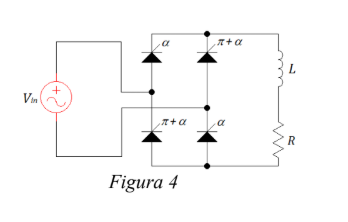
\includegraphics[width=0.6\textwidth]{circuito_rectificador_puente_controlado_figura4.png}
\caption{Rectificador controlado de la figura 4 (puente completo, $\alpha$ y $\pi+\alpha$).}
\end{figure}

\subsection{Soluci\'on Anal\'itica}

Los valores del circuito, obtenidos a partir de las literales asignadas
($a=3$, $b=9$, $c=3$), son:

\begin{align*}
a &= 3,\quad b = 9,\quad c = 3 \\
V_s &= 30(9+3) = 360\ \text{V} \\
f &= 60\ \text{Hz} \\
R &= (3+9+3)\ \Omega = 15\ \Omega \\
L &= 60\ \text{mH} \\
\alpha &= 90^\circ = 1{,}5708\ \text{rad}
\end{align*}

La constante de tiempo de la respuesta natural, la frecuencia angular y el
instante de disparo (retardo desde el cruce por cero) son:

\begin{align*}
\tau &=  \frac{60\times10^{-3}}{15\ \Omega} = 0{,}004\ \text{s} \\
\frac{1}{\tau} &= 250\ \text{s}^{-1} \\
\omega &= 2\pi(60\ \text{Hz}) = 376{,}991\ \text{rad/s} \\
t_1 &= \frac{1{,}5708}{376{,}991} = \boxed{4{,}1667\ \text{ms}}
\end{align*}

La respuesta forzada se obtiene con la impedancia de la carga a la
frecuencia de la fuente:

\begin{align*}
Z &= 15\ \Omega + j(120\pi)(60\times10^{-3}) = 15\ \Omega + j22{,}6195 \\
|Z| &= \sqrt{(22{,}6195)^2+(15)^2} = 27{,}14\ \Omega \\
\varphi &= \tan^{-1}\!\left(\frac{22{,}6195}{15}\right) = 0{,}98\ \text{rad} \\
Z &= 27{,}14\ \Omega \angle 0{,}98
\end{align*}

Con esta impedancia, la corriente fasorial forzada resulta:

\begin{align*}
V_m &= 360\ \text{V}\cdot\sqrt{2} = 509{,}12\ \text{V} \\
I_f &= \frac{509{,}12\ \text{V}\angle 0}{27{,}14\ \Omega\angle 0{,}98} = 18{,}76\ \text{A}\angle{-0{,}98}
\end{align*}

Esta corriente en funci\'on del tiempo, sumando la respuesta natural
(exponencial), es:

\begin{align*}
i(t) &= 18{,}76\,\sen(120\pi t - 0{,}98) + I_o\,e^{-250(t-0{,}0041667)}
\end{align*}

Con la condici\'on inicial en $t=t_1$ ($i(t_1)=0$) se calcula $I_o$ mediante:

\begin{align*}
0 &= 18{,}76\,\sen(1{,}5708 - 0{,}98) + I_o \\
I_o &= \boxed{-10{,}45\ \text{A}}
\end{align*}

\begin{figure}[H]
\centering
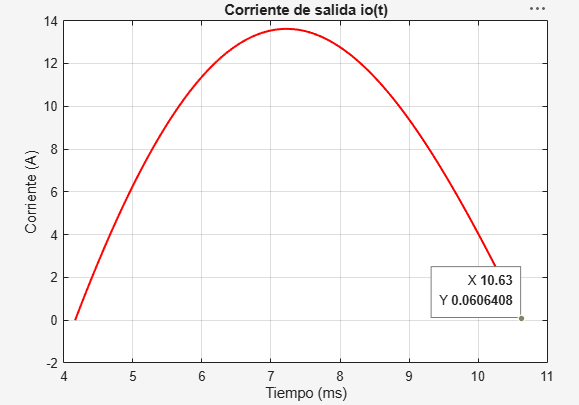
\includegraphics[width=0.6\textwidth]{ejercicio5_corriente_salida_io_alpha90.png}
\caption{Se\~nal de corriente $i(t)$.}
\end{figure}

En la Figura anterior se muestra la corriente del circuito; en la condici\'on
final se tiene que la corriente $i=0$ en $t=t_e$, con esta condici\'on se
eval\'ua el tiempo de extinci\'on:

\begin{align*}
0 &= 18{,}76\,\sen(120\pi\,t_e - 0{,}98) - 10{,}45\,e^{-250(t_e-0{,}0041667)}
\end{align*}

Con un tiempo inicial de c\'alculo de $9{,}5$~ms se obtiene $t_e$, y con \'este
el \'angulo de extinci\'on:

\begin{align*}
t_e &\approx 0{,}01063\ \text{s} = \boxed{10{,}63\ \text{ms}} \\
\beta &= 376{,}991\cdot 0{,}01063 = \boxed{4{,}01\ \text{rad}}
\end{align*}

Como $\beta = 4{,}01\ \text{rad} < \pi+\alpha = 4{,}71\ \text{rad}$
$\Rightarrow$ \textbf{la corriente es discontinua} (\'angulo de extinci\'on
$\beta=4{,}01$~rad, tipo de corriente: discontinua).

\subsection{Valores promedio y Eficaces de Tensiones y Corrientes}

El voltaje DC es:

\begin{align*}
V_{DC} &= \frac{1}{\pi}\int_{1{,}5708}^{4{,}01} 509{,}12\,\sen(\theta)\,d\theta
        = \frac{509{,}12}{\pi}\Big[-\cos(\theta)\Big]_{1{,}5708}^{4{,}01} \\
V_{DC} &= \frac{509{,}12}{\pi}\big[-\cos(4{,}01)+\cos(1{,}5708)\big]
        = \frac{509{,}12}{\pi}(0{,}6448+0) = \boxed{104{,}5\ \text{V}}
\end{align*}

La tensi\'on eficaz est\'a dada por:

\begin{align*}
V_{RMS}^2 &= \frac{1}{\pi}\int_{1{,}5708}^{4{,}01} \big[509{,}12\,\sen(\theta)\big]^2\,d\theta
           = \frac{509{,}12^2}{\pi}\left[\frac{\theta}{2}-\frac{\sen(2\theta)}{4}\right]_{1{,}5708}^{4{,}01} \\
V_{RMS}^2 &= \frac{509{,}12^2}{\pi}\big[(2{,}0055-0{,}2466)-(0{,}7854-0)\big]
           = 82486{,}5\cdot 0{,}9736 = 80302\ \text{V}^2 \\
V_{RMS} &= \sqrt{80302} = \boxed{283{,}4\ \text{V}}
\end{align*}

La corriente DC es:

\begin{align*}
I_{DC} &= \frac{2}{0{,}016667}\int_{0{,}0041667}^{0{,}01063}
          \Big[18{,}76\,\sen(120\pi t - 0{,}98) - 10{,}45\,e^{-250(t-0{,}0041667)}\Big]dt \\
I_{DC} &= \boxed{6{,}88\ \text{A}}
\end{align*}

La corriente eficaz est\'a dada por:

\begin{align*}
I_{RMS}^2 &= \frac{2}{0{,}016667}\int_{0{,}0041667}^{0{,}01063}
             \Big[18{,}76\,\sen(120\pi t - 0{,}98) - 10{,}45\,e^{-250(t-0{,}0041667)}\Big]^2 dt \\
I_{RMS}^2 &= 74{,}14\ \text{A}^2 \quad\Rightarrow\quad I_{RMS} = \sqrt{74{,}14} = \boxed{8{,}61\ \text{A}}
\end{align*}

\subsection{Potencias Activa y aparente}

\begin{align*}
P &= 74{,}14 \cdot 15 = \boxed{1112{,}1\ \text{W}} \\
P_{DC} &= 104{,}5 \cdot 6{,}88 = \boxed{719{,}0\ \text{W}} \\
S &= 360 \cdot 8{,}61 = \boxed{3099{,}6\ \text{VA}}
\end{align*}

\subsection{Par\'ametros de Rendimiento}

\begin{align*}
FP &= \frac{1112{,}1}{3099{,}6} = \boxed{0{,}359} \\
\eta &= \frac{719{,}0}{3099{,}6} = \boxed{0{,}232}
\end{align*}

\begin{align*}
FR_V &= \frac{\sqrt{283{,}4^2 - 104{,}5^2}}{104{,}5} = \boxed{2{,}52} \\
FR_I &= \frac{\sqrt{8{,}61^2 - 6{,}88^2}}{6{,}88} = \boxed{0{,}753}
\end{align*}

\subsection{Dibujo de Se\~nales}

\subsubsection{Definiciones}

La se\~nal de tensi\'on de salida est\'a dada por:
\begin{align*}
v_o(t) = \begin{cases} 509{,}12\,\sen(120\pi t) & \text{si } t_1 \le t < t_e \\ 0 & \text{si } t_e \le t < t_1+T/2 \end{cases}
\end{align*}

Mientras que la funci\'on de corriente es:
\begin{align*}
i_o(t) = \begin{cases} 18{,}76\,\sen(120\pi t - 0{,}98) - 10{,}45\,e^{-250(t-0{,}0041667)} & \text{si } t_1 \le t < t_e \\ 0 & \text{si } t_e \le t < t_1+T/2 \end{cases}
\end{align*}

\subsubsection{C\'odigo}

El c\'odigo en MatLab para realizar las gr\'aficas de las se\~nales es:

\begin{lstlisting}[language=Matlab, caption={C\'odigo MATLAB -- $v_o(t)$, Ejercicio 5}, label={lst:ex5vo}]
x=linspace(0.0041667,0.01063,200);
vo=509.12*sin(376.991*x);
plot(x*1e3,vo,'b','LineWidth',1.5); hold on
title('Tension de salida vo(t)'); xlabel('Tiempo (ms)'); ylabel('Tension (V)')
grid on
\end{lstlisting}

\begin{lstlisting}[language=Matlab, caption={C\'odigo MATLAB -- $i_o(t)$, Ejercicio 5}, label={lst:ex5io}]
x=linspace(0.0041667,0.01063,200);
io=18.76*sin(376.991*x-0.98)-10.45*exp(-250*(x-0.0041667));
plot(x*1e3,io,'r','LineWidth',1.5); hold on
title('Corriente de salida io(t)'); xlabel('Tiempo (ms)'); ylabel('Corriente (A)')
grid on
\end{lstlisting}

\subsubsection{Gr\'aficas Resultantes}

\begin{figure}[H]
\centering
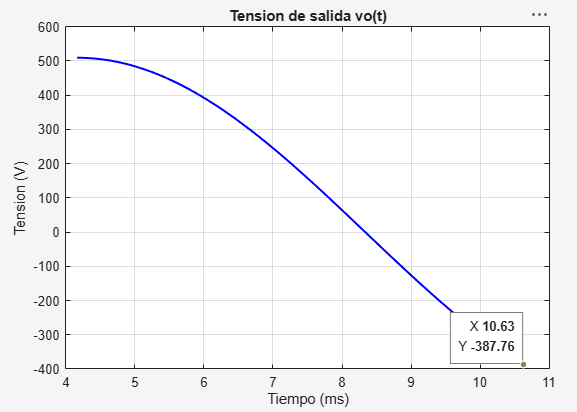
\includegraphics[width=0.75\textwidth]{ejercicio5_tension_salida_vo_alpha90.png}
\caption{Tensi\'on de salida $v_o(t)$ -- Ejercicio 5 ($\alpha=90^\circ$, corriente discontinua).}
\end{figure}

\begin{figure}[H]
\centering
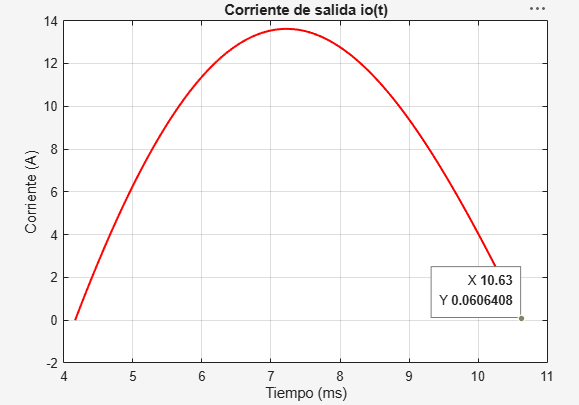
\includegraphics[width=0.75\textwidth]{ejercicio5_corriente_salida_io_alpha90.png}
\caption{Corriente de salida $i_o(t)$ -- Ejercicio 5 ($\alpha=90^\circ$, corriente discontinua).}
\end{figure}

\subsection{Simulaciones}

Se simul\'o el puente completo controlado (T1-T4, con los mismos retardos de
disparo $t_1$ y $(\pi+\alpha)/\omega$) en Simscape Electrical, con
$V_{in}=509{,}12$~V, $R=15\,\Omega$, $L=60$~mH.

\subsubsection{Mediciones de tensiones y corrientes}

\begin{figure}[H]
\centering
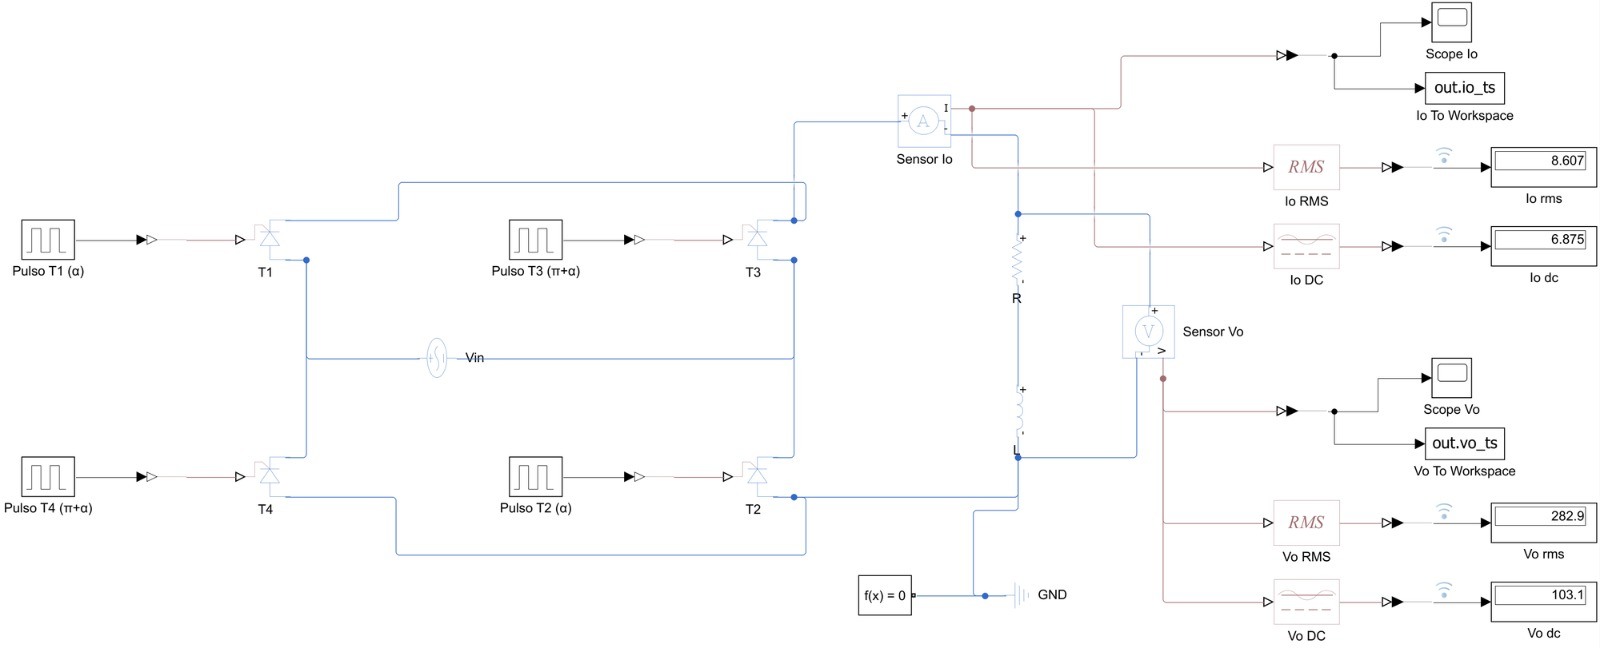
\includegraphics[width=\textwidth]{simulacion_simulink_scr_puente_p5_resultados.png}
\caption{Modelo Simscape Electrical del puente completo controlado (T1-T4) con los sensores de $I_o$ y $V_o$ y los indicadores de RMS/DC obtenidos.}
\label{fig:sim5}
\end{figure}

Los sensores de la Figura~\ref{fig:sim5} arrojan directamente:
\begin{align*}
V_{DC,sim} = 103{,}1\ \text{V}, \quad V_{RMS,sim} = 282{,}9\ \text{V}, \quad
I_{DC,sim} = 6{,}875\ \text{A}, \quad I_{RMS,sim} = 8{,}607\ \text{A}
\end{align*}

\subsubsection{Se\~nales De Simulaci\'on}

En la Figura~\ref{fig:vosim5} se muestra la se\~nal de tensi\'on de la
simulaci\'on, con el periodo completo (incluyendo el tramo en cero propio de
la corriente discontinua) y el tiempo de extinci\'on marcado; en la
Figura~\ref{fig:iosim5} se aprecia la se\~nal de corriente correspondiente.

\begin{figure}[H]
\centering
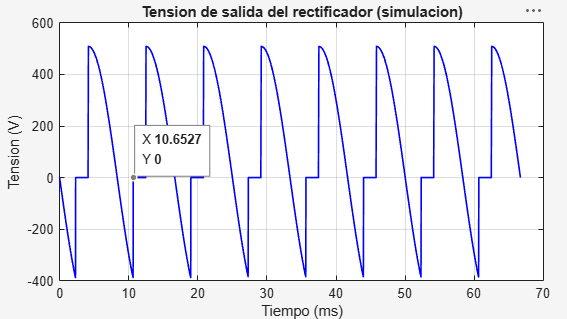
\includegraphics[width=0.8\textwidth]{ejercicio5_simulacion_vo_periodo_completo.png}
\caption{Tensi\'on de salida del rectificador (simulaci\'on, periodo completo).}
\label{fig:vosim5}
\end{figure}

\begin{figure}[H]
\centering
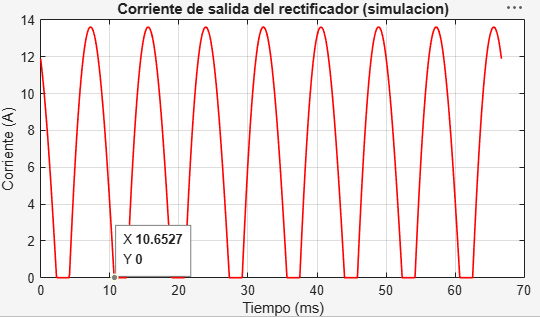
\includegraphics[width=0.8\textwidth]{ejercicio5_simulacion_io_periodo_completo.png}
\caption{Corriente de salida del rectificador (simulaci\'on, periodo completo).}
\label{fig:iosim5}
\end{figure}

\subsection{C\'alculos con los Datos de Simulaci\'on}

En la simulaci\'on se obtuvieron estos resultados (ver Figura~\ref{fig:sim5}):

\begin{align*}
V_{DC,sim} = 103{,}1\ \text{V}, \quad V_{RMS,sim} = 282{,}9\ \text{V}, \quad
I_{DC,sim} = 6{,}875\ \text{A}, \quad I_{RMS,sim} = 8{,}607\ \text{A}
\end{align*}

Con estos datos se procede a realizar los c\'alculos de todos los dem\'as
par\'ametros as\'i:

\begin{align*}
P_{sim} &= 8{,}607^2 \cdot 15 = \boxed{1111{,}2\ \text{W}} \\
P_{DC,sim} &= 103{,}1 \cdot 6{,}875 = \boxed{708{,}8\ \text{W}} \\
S_{sim} &= 360 \cdot 8{,}607 = \boxed{3098{,}5\ \text{VA}}
\end{align*}

\begin{align*}
FP_{sim} &= \frac{1111{,}2}{3098{,}5} = \boxed{0{,}359} \\
\eta_{sim} &= \frac{708{,}8}{3098{,}5} = \boxed{0{,}229}
\end{align*}

\begin{align*}
FR_{V,sim} &= \frac{\sqrt{282{,}9^2 - 103{,}1^2}}{103{,}1} = \boxed{2{,}56} \\
FR_{I,sim} &= \frac{\sqrt{8{,}607^2 - 6{,}875^2}}{6{,}875} = \boxed{0{,}753}
\end{align*}

\subsection{Comparaci\'on de Resultados}

\begin{center}
\begin{tabular}{c c c c}
Par\'ametro & Valor Calculado & Valor de Simulaci\'on & Error (\%) \\ \hline
$t_e$ (ms) & 10{,}63 & 10{,}6527 & 0{,}21 \\
$V_{DC}$ (V) & 104{,}5 & 103{,}1 & 1{,}34 \\
$V_{RMS}$ (V) & 283{,}4 & 282{,}9 & 0{,}18 \\
$I_{DC}$ (A) & 6{,}88 & 6{,}875 & 0{,}07 \\
$I_{RMS}$ (A) & 8{,}61 & 8{,}607 & 0{,}04 \\
$P$ (W) & 1112{,}1 & 1111{,}2 & 0{,}08 \\
$S$ (VA) & 3099{,}6 & 3098{,}5 & 0{,}04 \\
$fp$ & 0{,}359 & 0{,}359 & 0{,}00 \\
$\eta$ & 0{,}232 & 0{,}229 & 1{,}38 \\
$FR_V$ & 2{,}52 & 2{,}56 & 1{,}43 \\
$FR_I$ & 0{,}753 & 0{,}753 & 0{,}01 \\
\end{tabular}
\end{center}

Todos los errores est\'an por debajo del $1{,}5\%$, muy por debajo del
$5\%$ t\'ipico esperado.

\end{document}
